\documentclass{article}
\usepackage{tikz}
\usetikzlibrary{shapes.multipart, positioning, arrows.meta}
\usepackage[margin=0.5in]{geometry}

\begin{document}
\begin{figure}[htbp]
\centering
\vspace{1cm}
\resizebox{\textwidth}{!}{
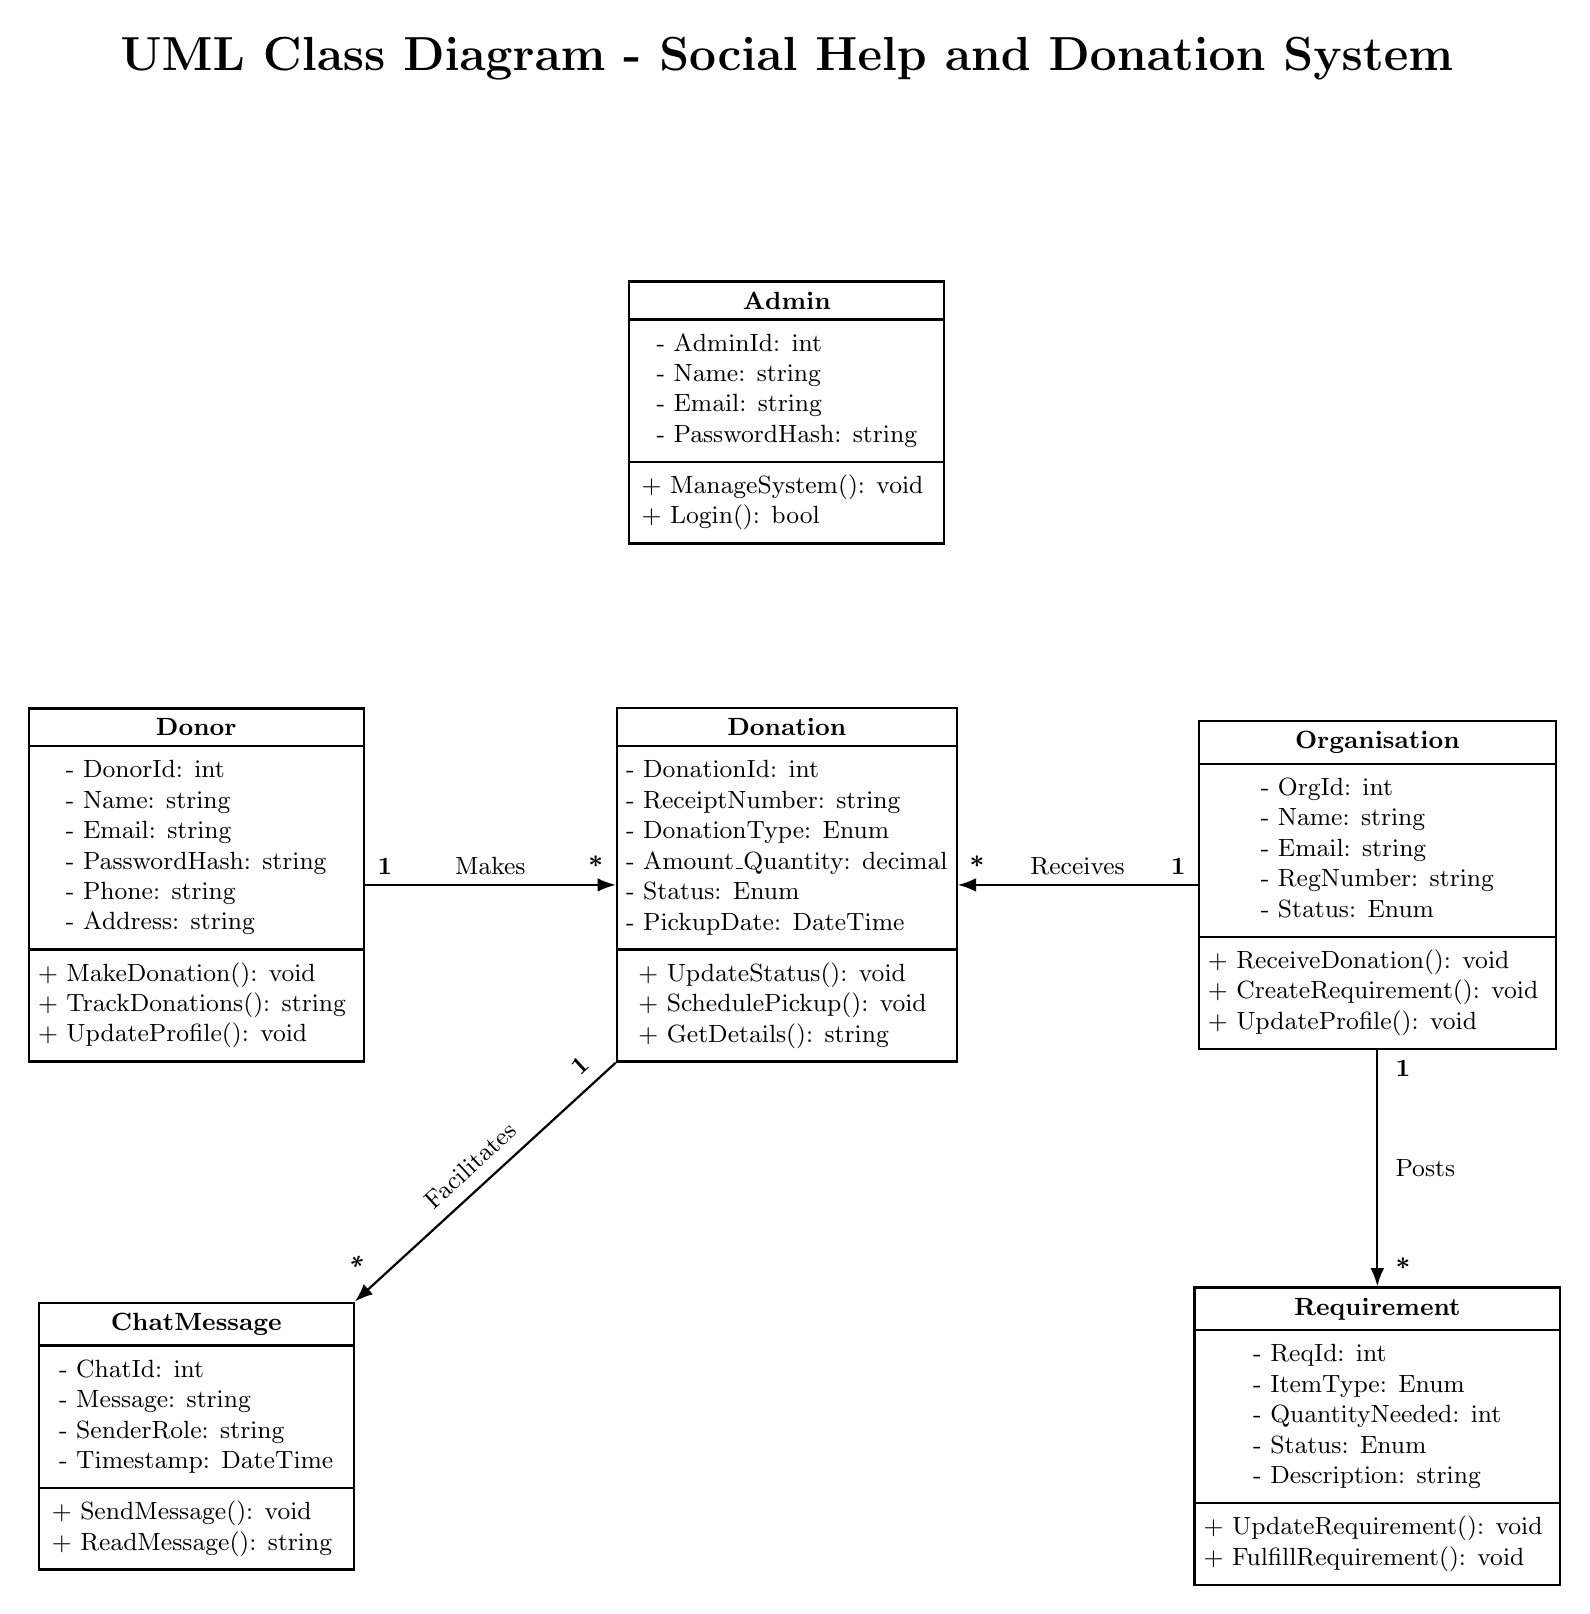
\begin{tikzpicture}[
    >=Latex,
    class/.style={
        draw=black, rectangle split, rectangle split parts=3,
        minimum width=4cm, align=center, fill=white, thick, font=\small
    }
]

% Title
\node[font=\LARGE\bfseries, align=center] at (0, 10.5) {UML Class Diagram - Social Help and Donation System};

% -------------------------
% Class Nodes Definition
% -------------------------

% 1. Admin (Top Center)
\node[class] (Admin) at (0, 6) {
    \textbf{Admin}
    \nodepart{second}
    \normalfont
    \begin{tabular}{@{}l@{}}
    - AdminId: int \\
    - Name: string \\
    - Email: string \\
    - PasswordHash: string
    \end{tabular}
    \nodepart{third}
    \normalfont
    \begin{tabular}{@{}l@{}}
    + ManageSystem(): void \\
    + Login(): bool
    \end{tabular}
};

% 2. Donation (Center)
\node[class] (Donation) at (0, 0) {
    \textbf{Donation}
    \nodepart{second}
    \normalfont
    \begin{tabular}{@{}l@{}}
    - DonationId: int \\
    - ReceiptNumber: string \\
    - DonationType: Enum \\
    - Amount\_Quantity: decimal \\
    - Status: Enum \\
    - PickupDate: DateTime
    \end{tabular}
    \nodepart{third}
    \normalfont
    \begin{tabular}{@{}l@{}}
    + UpdateStatus(): void \\
    + SchedulePickup(): void \\
    + GetDetails(): string
    \end{tabular}
};

% 3. Donor (Left)
\node[class] (Donor) at (-7.5, 0) {
    \textbf{Donor}
    \nodepart{second}
    \normalfont
    \begin{tabular}{@{}l@{}}
    - DonorId: int \\
    - Name: string \\
    - Email: string \\
    - PasswordHash: string \\
    - Phone: string \\
    - Address: string
    \end{tabular}
    \nodepart{third}
    \normalfont
    \begin{tabular}{@{}l@{}}
    + MakeDonation(): void \\
    + TrackDonations(): string \\
    + UpdateProfile(): void
    \end{tabular}
};

% 4. Organisation (Right)
\node[class] (Org) at (7.5, 0) {
    \textbf{Organisation}
    \nodepart{second}
    \normalfont
    \begin{tabular}{@{}l@{}}
    - OrgId: int \\
    - Name: string \\
    - Email: string \\
    - RegNumber: string \\
    - Status: Enum
    \end{tabular}
    \nodepart{third}
    \normalfont
    \begin{tabular}{@{}l@{}}
    + ReceiveDonation(): void \\
    + CreateRequirement(): void \\
    + UpdateProfile(): void
    \end{tabular}
};

% 5. Requirement (Bottom Right)
\node[class] (Requirement) at (7.5, -7) {
    \textbf{Requirement}
    \nodepart{second}
    \normalfont
    \begin{tabular}{@{}l@{}}
    - ReqId: int \\
    - ItemType: Enum \\
    - QuantityNeeded: int \\
    - Status: Enum \\
    - Description: string
    \end{tabular}
    \nodepart{third}
    \normalfont
    \begin{tabular}{@{}l@{}}
    + UpdateRequirement(): void \\
    + FulfillRequirement(): void
    \end{tabular}
};

% 6. ChatMessage (Bottom Left)
\node[class] (Chat) at (-7.5, -7) {
    \textbf{ChatMessage}
    \nodepart{second}
    \normalfont
    \begin{tabular}{@{}l@{}}
    - ChatId: int \\
    - Message: string \\
    - SenderRole: string \\
    - Timestamp: DateTime
    \end{tabular}
    \nodepart{third}
    \normalfont
    \begin{tabular}{@{}l@{}}
    + SendMessage(): void \\
    + ReadMessage(): string
    \end{tabular}
};

% -------------------------
% Path Connections & Multiplicities
% -------------------------

% Donor -> Donation
\draw[->, thick] (Donor.east) -- (Donation.west) 
    node[pos=0.08, above, font=\small\bfseries] {1} 
    node[midway, above, font=\small] {Makes} 
    node[pos=0.92, above, font=\small\bfseries] {*};

% Org -> Donation
\draw[->, thick] (Org.west) -- (Donation.east) 
    node[pos=0.08, above, font=\small\bfseries] {1} 
    node[midway, above, font=\small] {Receives} 
    node[pos=0.92, above, font=\small\bfseries] {*};

% Org -> Requirement
\draw[->, thick] (Org.south) -- (Requirement.north) 
    node[pos=0.08, right=0.1cm, font=\small\bfseries] {1} 
    node[midway, right=0.1cm, font=\small] {Posts} 
    node[pos=0.92, right=0.1cm, font=\small\bfseries] {*};

% Donation -> ChatMessage (Diagonal)
\draw[->, thick] (Donation.south west) -- (Chat.north east) 
    node[pos=0.08, sloped, above=0.05cm, font=\small\bfseries] {1} 
    node[midway, sloped, above=0.05cm, font=\small] {Facilitates} 
    node[pos=0.92, sloped, above=0.05cm, font=\small\bfseries] {*};

\end{tikzpicture}
}
\end{figure}
\end{document}
